\chapter{布局}

\begin{quotation}
离娄之明,公输子之巧,不以规矩,不能成方圆。
\begin{flushright}
--- 《孟子·离娄上》
\end{flushright}
\end{quotation}

我们在 \ref{sec:box} 节中曾经提到,在 \LaTeX 中每一个排版对象都是一个盒子。排版就是要把小盒子用空白间距粘在一起放到大盒子里,然后再依次嵌套到更大的盒子里。怎样优化这些大大小小的盒子是一门很深的学问,在本章里我们将会略窥门径。

\section{页面尺寸}

在排版时页面是最大的盒子,所以我们就先看一看它。人们在日常生活中可以见到多种规格的纸张,它们一般归属于两大类标准:公制和美制。

\subsection{普通青年}

早在1786年,德国科学家 Georg C. Lichtenberg (1742--1799)\indexLichtenberg 就发现$1/\sqrt{2}$这个比例可以用于分割纸张。你拿一张这个比例的纸,在较长的那个方向上一分为二,得到的两张纸也是同样比例。

1912--1914年间,另一个德国人 Walter Porstmann (1886--1959)\indexPorstmann 在为诺贝尔化学奖得主 Wilhelm Ostwald (1853--1932)\indexOstwald{} \footnote{生于拉脱维亚,1878年塔图大学 (University of Tartu) 博士,1909年诺贝尔化学奖。}当助手时,两人企图把这个比例变成一个世界标准。一个数学家和一个化学家在一起琢磨这个好像不务正业,但是考虑到 Ostwald 当时还兼任一个知识产权研究所的主任,好歹也沾点边儿。他们从 1cm x 1.41cm 开始,每次加倍短边,直至无穷。然而他们的提议无人理会,也许人们都正忙于第一次世界大战。此后几年 Porstmann 一直沿着这个方向灌水,甚至他在1918年写的博士论文也与此相关。

当时德国标准化学会 (Deutsches Institut für Normung, DIN)\index{org}{org.din@Deutsches Institut für Normung, DIN, 德国标准化学会} 刚成立没多久,无所事事的学会领导 Waldemar Hellmich\indexHellmich 注意到了 Porstmann,就在1920年将其网罗至门下。1922年,DIN 发布了476纸张标准,这次是从面积一平方米的 A0 (841mm × 1189mm)开始,每次减半长边。后来又陆续加上了 B, C, D 系列。

DIN 476 因为其简单易用,逐渐流行到其他国家。1961年 ISO 将 A 和 B 系列采纳为推荐标准,1975年变成 ISO 216 标准。其中 B 系列比 DIN 476 的略大一点,它从 1000mm × 1414mm 的 B0 开始。1985年发布的 ISO 269 加上了 C 系列,它的尺寸是 A 和 B 系列纸张尺寸的几何平均。

A 系列常用于公文;B 系列常用于海报和护照 (B7, 88mm × 125mm);C 系列常用于信封,因为它恰好比 A 系列大一点,比如 A4 纸可以装在 C4 信封里,对折一下就可以装进 C5 信封,再对折一次装进 C6 信封。

\subsection{文二青年}

当今世界大多数国家都采用此项国际标准,冥顽不化的只有美国和它的几个小弟,在这些地方流行的是比 A4 胖一点的 Letter (8.5in × 11in) 。Letter 追溯上去应该源于大英帝国,只是英国在1950年代末就已经全面接受了公制标准。窃以为一小撮美洲人对英制情有独钟的原因是他们的历史短,所以但凡有把年纪的东西都颇为珍惜。

IEEE\indexIEEE{}定义过一个Government-Letter (8in × 10.5in) ,主要用于儿童读物。想来儿童读的东西信息量少,不需要 Letter 那么大的纸。Herbert\linebreak Hoover (1874--1964)\indexHoover{} \footnote{美国第31任总统,历任总统中罕见的工科 WSN。1895年斯坦福地质学士,自称是该校首名学生。在校期间曾担任棒球队经理,向前总统 Benjamin Harrison 追讨两毛五门票钱。} 在1920年代担任商务部长期间,规定政府公文也采用此规格。我今天量过《时代周刊》和《商业周刊》,也是这个规格。

1980年代初Ronald Reagan (1911--2004)\indexReagon{} 上台后,认为美利坚乃天朝上国,用小纸太丢脸,于是政府公文改用 Letter。我对 Letter 没啥意见,在写本章之前用的就是它,现在改用 A4 是为了照顾中文读者的习惯。坑爹的是 Legal (8.5in × 14in) ,比普通文件夹都长一大截,它主要用于法律文件。

面对世界标准化潮流,老美的颜面有点 hold 不住,于是在1996年推出 ANSI Y14.1 作为遮羞布。它定义了 A, B, C, D, E 五种规格,A 就是 Letter,B 比A 面积大一倍,C 比 B 大一倍,依次类推。它们的长宽比不一致,B 和 C 比其他三种瘦很多。它们的尺寸倒是和 A4--A0 差不多,如果不挑剔也可以混用。

\subsection{尺寸详解}

\begin{figure}[!htbp]
\centering
\includegraphics[page=24]{pgf.pdf}
\caption{页面尺寸}
\label{fig:pagelayout}
\end{figure}

\autoref{fig:pagelayout} 是一张 A4,尺寸为 210mm × 297mm 也就是 597pt × 845pt。图中标注为 Body 的是正文区域,Header 是页眉,Footer 是页脚。图中标注的尺寸有些是固定的,另一些是随着正文字号或其他因素而改变的;在这里我们会遇到一些 \LaTeX 定义的尺寸宏变量。

lshort 里有张类似的图流传甚广,包老师为了操练一把20年前学到的机械制图本领,就自己画了一张。图中尺寸用的是 11pt,oneside 的,下面我们就以此为例介绍一下这些尺寸:

\begin{enumerate}
  \item 页边距,1in。在微软Word里这个尺寸也很常见;
  \item \verb|\oddsidemargin| 或 \verb|\evensidemargin|,奇数或偶数页左边距,46pt;
  \item \verb|\textwidth|,正文宽度,360pt,可以放下大概32个汉字;
  \item 597pt减去左边的 1in + 46pt 和中间的 360pt,还剩下 119pt,左右相差不到 1pt。如果双面打印的话,两面的正文部分恰好是重叠的;
  \item 页边距,1in;
  \item \verb|\topmargin|,上边距,18pt;
  \item \verb|\headheight|,页眉高度,12pt;
  \item \verb|\headsep|,页眉与正文间距,25pt;
  \item \verb|\textheight|,正文高度,595pt,可以放下38行文字;
  \item \verb|\footskip|,正文与页脚基线间距,30pt。它比页眉的 12pt + 25pt 小了 7pt,不理解的同学可以照照镜子,你左右是对称的,但是上下呢?
  \item 845pt 减去上面全部尺寸,还剩下 93pt,比上面的 1in + 18pt 多了 3pt。
\end{enumerate}

当字号等发生变化时,上述某些尺寸也会发生一定的变化。比如我们把 oneside 改成 twoside,那么奇偶页的左边距就分别变成 22pt 和 70pt。但是奇数页右边空白恰好和偶数页左边空白相等,不会给双面打印造成困扰。

一般情况下我们无须改动 \LaTeX 的页面布局缺省设置。当有特殊需要时,可以使用 \ref{sec:length} 节提到的 \verb|\setlength| 或 \verb|\addtolength| 来设置上述宏变量的值。

梅木秀雄\indexUmeki{} \footnote{东芝高级经理。}的 \texttt{geometry} 宏包\citep{Umeki_geometry}则提供了更高级的用户接口。比如我们可以用如下的方法来设置页面尺寸和边距,

\begin{Code}[]
\usepackage[paperwidth=100mm, paperheight=150mm, margin=20mm]{geometry}
\end{Code}

也可以像下面这样单独设置每个边距,

\begin{Code}[]
\usepackage[top=2in, bottom=1in, left=1in, right=1in]{geometry}
\end{Code}

想把页面横过来,可以这样,

\begin{Code}[]
\usepackage[landscape]{geometry}
\end{Code}

\section{页面样式}

了解页面尺寸之后,我们再来看看页面样式,也就是页眉和页脚的内容。\LaTeX 预定义了四种样式,见 \autoref{tab:pagestyle}。

\begin{table}[htbp]
\caption{\LaTeX 页面样式}
\label{tab:pagestyle}
\centering
\begin{tabular}{ll}
  \toprule
  \texttt{empty} & 页眉、页脚空白 \\
  \texttt{plain} & 页眉空白,页脚含居中页码,非book文档类缺省值 \\
  \texttt{headings} & 页脚空白,页眉含章节名和页码,book文档类缺省值 \\
  \texttt{myheadings} & 页脚空白,页眉含页码和用户自定义信息 \\
  \bottomrule
\end{tabular}
\end{table}

我们可以用 \verb|\pagestyle| 和 \verb|\thispagestyle| 命令来设置整个文档或单独某页的样式。

\begin{Code}[numbers=none]
\pagestyle{plain}    %全局设置
\thispagestyle{empty}%单页设置
\end{Code}

\autoref{tab:pagestyle} 中的样式是通过重定义四个宏变量 \texttt{@oddhead}, \texttt{@evenhead}, \texttt{@oddfoot}, \texttt{@evenfoot} 来设置奇偶页的页眉与页脚。

我们也可以用 \autoref{exa:def_pagestyle} 中的方法来自定义样式。其中第2行代码定义了 \texttt{permanentdamagedhead} 样式,定义这个特殊命令时,一定要写成 \verb|\ps@style| 的样子;而在引用时,则写成 \verb|\pagestyle{style}|。第3--6行分别定义了奇偶页的页眉和页脚;单面文档奇偶页样式一样,所以需要且只需要定义奇数页的页眉和页脚,偶数页的定义不起作用。

\begin{example}[htbp]
\LoadFBTDemo[]{texlet/layout-pagestyle}
\LoadDemo{texlet/layout-pagestyle-a}
\caption{自定义页面样式}
\label{exa:def_pagestyle}
\end{example}

这段代码中的 \verb|\hfill| 是个弹性填充命令,它把两边的内容“推”得尽可能远。例中使用了特殊符号 \texttt{@},所以要在第一行用 \verb|\makeatletter| 命令声明一下,暂时把它当正常符号用;用完之后,在最后一行用相应的 \verb|\makeatother| 命令恢复现场。

在自定义页面样式时,我们不仅可以在页眉和页脚里使用普通字符串,也可以使用一些宏变量来显示页码、章节号码和名称等(见 \autoref{tab:pagestyle_macro})。

\begin{table}[!h]
\centering
\caption{页眉和页脚常用宏变量}
\label{tab:pagestyle_macro}
\begin{tabularx}{350pt}{lX}
  \toprule
  \verb|\thepage| & 页码 \\
  \verb|\thechapter| & 章编号 \\
  \verb|\thesection| & 节编号 \\
  \verb|\chaptername| & 章起始单词名,Chapter \\
  \verb|\sectionname| & 节起始单词名,Section \\
  \verb|\leftmark| & 左标记,在 \texttt{article} 文档类中包含 \texttt{section} 信息,在 \texttt{report} 和 \texttt{book} 中则包含 \texttt{chapter} 信息。\\
  \verb|\rightmark| & 右标记,在 \texttt{article} 中包含 \texttt{subsection} 信息,在 \texttt{report} 和 \texttt{book} 中则包含 \texttt{section} 信息。\\
  \bottomrule
\end{tabularx}
\end{table}

\autoref{tab:pagestyle_macro} 中前五个变量都可以直接重定义,左右标记特殊一点,需要用下面的命令来间接定义,

\begin{Code}[numbers=none]
\markboth{`左标记`}{`右标记`}%定义两个标记
\markright{`右标记`}      %定义右标记
\end{Code}

需要注意的是,引用时要用 \verb|\leftmark| 和 \verb|\rightmark|,定义时要用 \verb|\markboth| 和 \verb|\markright|。为什么会这样呢?因为 Lamport 是个怪叔叔。另外为什么没有 \verb|\markleft| 呢?其实这个命令在AMS的几个文档类里是有的。这个故事告诉我们:AMS 是左派进步青年,Lamport 是右倾分子,所以他后来脱离革命加入了微软。

\autoref{exa:headings} 是 \texttt{book} 文档类中双面打印时 \texttt{headings} 样式定义的节选。其中第2行清空页脚;第3行定义偶数页(也就是左页)页眉,页码居左,左标记居右;第4行定义奇数页(右页)页眉,右标记居左,页码居右。这样页码总是在书的外侧,便于阅读时翻页定位。 

\begin{example}[htbp]
\begin{Code}[]
\def\ps@headings{%
  \let\@oddfoot\@empty\let\@evenfoot\@empty
  \def\@evenhead{\thepage\hfill\slshape\leftmark}%
  \def\@oddhead{{\slshape\rightmark}\hfill\thepage}%
  ...
\end{Code}
\caption{\texttt{headings} 样式}
\label{exa:headings}
\end{example}

\autoref{exa:myheadings} 则是 \texttt{book} 文档类中 \texttt{myheadings} 样式的定义。只看前四行它好像和 \texttt{headings} 样式是孪生兄弟,差别在于下面三行清空了左右标记,用户需要自行定义,否则偶数页右上角和奇数页左上角是空白的。

\begin{example}[htbp]
\begin{Code}[]
\def\ps@myheadings{%
  \let\@oddfoot\@empty\let\@evenfoot\@empty
  \def\@evenhead{\thepage\hfill\slshape\leftmark}%
  \def\@oddhead{{\slshape\rightmark}\hfill\thepage}%
  \let\@mkboth\@gobbletwo
  \let\chaptermark\@gobble
  \let\sectionmark\@gobble
}
\end{Code}
\caption{\texttt{myheadings} 样式}
\label{exa:myheadings}
\end{example}

\autoref{exa:markboth} 演示了怎样为 \texttt{myheadings} 样式定制左右标记。写到这里包老师忽然想到,好像东西方文化在左比右高级这一点上是一致的,文东武西,男左女右。正因为如此阳顶天挂了之后杨逍可以去泡妞,而范遥只能毁了容去卧底,思想境界上还是差那么一点点。

\begin{example}[htbp]
\LoadFBTDemo[]{texlet/layout-markboth}
\LoadDemo{texlet/layout-markboth-a}
\caption{定制左右标记}
\label{exa:markboth}
\end{example}

用户可能会觉得上述定义页面样式的方法比较繁琐和低级,Piet van Oostrum\indexOostrum{} \footnote{曾任教于荷兰乌德勒支大学(Utrecht University),退休后隐居于南美。}的 \texttt{fancyhdr} 宏包\citep{Oostrum_fancyhdr}则提供了更灵活的控制和高级的语法。

\begin{example}[htbp]
\LoadFBTDemo[]{texlet/layout-fancyhdr}
\caption{\texttt{fancyhdr} 宏包}
\label{exa:fancyhdr}
\end{example}

在 \autoref{exa:fancyhdr} 的代码中,第3行将页面样式设置为 \texttt{fancyhdr} 宏包定义的 \texttt{fancy} 样式;第4--9行分别定制了页眉和页脚;最后两行定制了页眉下方和页脚上方的横线。

左右标记里除了页码,通常还会有章节编号和名称等,这时我们就要用到另两个命令 \verb|\chaptermark| 和 \verb|\sectionmark|,其用法见 \autoref{exa:chaptermark}。

在这段代码中,第3行清空了页眉和页脚;第4行将页码置于偶数页左上和奇数页右上,第5行将左标记置于偶数页右上,第6行将右标记置于奇数页左上。

\begin{example}[htbp]
\LoadFBTDemo[]{texlet/layout-chaptermark}
\LoadDemo{texlet/layout-chaptermark-a}
\caption{定制章节标记}
\label{exa:chaptermark}
\end{example}

\texttt{fancyhdr} 宏包将每章起始页的样式设为 \texttt{plain},若想去掉页脚中间的页码,可以重定义 \texttt{plain} 样式。代码第7--10行清空了 \texttt{plain} 页的页眉和页脚,还去掉了页眉下方的横线。

第11行重定义了章标记,它传给 \verb|\markboth| 命令的参数是章的名称,这样章名就会出现在左标记里。章名最初是从哪里来的呢?它是用 \verb|\chapter{章名}| 命令定义的。章名从 \verb|\chapter| 传到 \verb|\chaptermark|,再传到 \verb|\markboth|,最后到了 \verb|\leftmark| 那里。它这样一路走来,不畏艰险,踏平坎坷,战胜妖魔,最终修成正果。

类似地,第12行重定义了节标记,它传给 \verb|\markright| 命令的参数是节的名称,这样节名就会出现在右标记里。

\section{分栏}

我们经常看到一些期刊报纸使用两栏或更多的栏位,这样可以节省空间和方便阅读。 \LaTeX 的标准文档类都有一个选项来支持双栏,

\begin{Code}[numbers=none]
\documentclass[twocolumn]{article}
\end{Code}

Mittelbach\indexMittelbach 的 \texttt{multicol} 宏包提供了更多的功能,比如它支持多达十个栏位,栏位数目可以任意切换;各栏长度相同,最后一页看起来会左右平衡一些。

\autoref{exa:cols} 中第2行代码将栏位之间的距离设为 12pt(缺省是 10pt),第3行将栏位之间的分割线宽度设为 1pt(缺省 0pt,也就是不显示);下面几行使用了 \texttt{multicols} 环境,注意环境名和宏包名是不同的。

\begin{example}[htbp]
\LoadFBTDemo[]{texlet/layout-cols}
\caption{\texttt{multicol} 宏包}
\label{exa:cols}
\end{example}

\texttt{multicols} 环境对浮动体的支持有限,只能使用带 \texttt{*} 的版本,见 \autoref{exa:starred_float}。这种特殊浮动体是跨栏位的,而且它们的 \texttt{h} 选项会失效,也就是不会出现在当前页。不管你的期望是多么地殷切,它最早也只能出现在下一页的页首。

\begin{example}[htbp]
\begin{Code}[]
\begin{figure*}[tbp]
...
\end{figure*}

\begin{table*}[tbp]
...
\end{table*}
\end{Code}
\caption{特殊浮动体}
\label{exa:starred_float}
\end{example}

某些权宜之计可以让浮动体出现在某栏内,但是它们就失去了浮动性,所以此处不赘述。

\section{分页}

\TeX 通常都会自动分页,无须人工干涉。但是浮动体较多的情况下,分页就变成一个 NP 完全问题 \footnote{传说 Knuth 在2046年写完那套书后,才会有时间改进分页算法。},自动分页的效果可能不是我们想要的。这时就需要手工插入分页命令,

\begin{Code}[numbers=none]
\newpage
\end{Code}

如果我们也不确定某处分页是否妥当,可以使用另一个命令,给 \TeX 留点面子。这个参数取值1--4,4表示强烈要求分页,1表示你看着办吧。

\begin{Code}[numbers=none]
\pagebreak[3]
\end{Code}

类似地,我们还可以建议 \TeX 不要分页,其参数取值也是1--4,4表示强烈反对分页,1表示随便。

\begin{Code}[numbers=none]
\nopagebreak[2]
\end{Code}

浮动体较多,\TeX 无所适从时,我们可以用下面的命令帮它减轻点责任。此命令要求 \TeX 排完此前所有浮动体,不管是否难看,咱就这么办了。

\begin{Code}[numbers=none]
\clearpage
\end{Code}

\bibliographystyle{unsrtnat}
\bibliography{lnotes2}
